\chapter{Intel Trusted Domain Extensions}

\section{Introduction}

\subsection{Confidential computing and intel TDX}

The aim of Confidential computing is rovide  protection for data in the enterprise and cloud environment (data in use). \\
Intel SGX is the first solution from Intel, and introduced the ability for user applications to run
computations in a protected memory space, creating a division between platform provider and other tenants (enclaves). This paradigm is called confidential computing.
Intel TDX is an architectural technology to deploy hardware-isolated VMS called Trusted Domains, isolated from the Virtual Machine Manager, Hypervisor and other non-TD software on the host platform. \\
Intel TDX was introduced in 2021 and was included in Intel's 4th Generation Xeon Scalable Processors in 2023.

\begin{figure}[H]
    \centering
    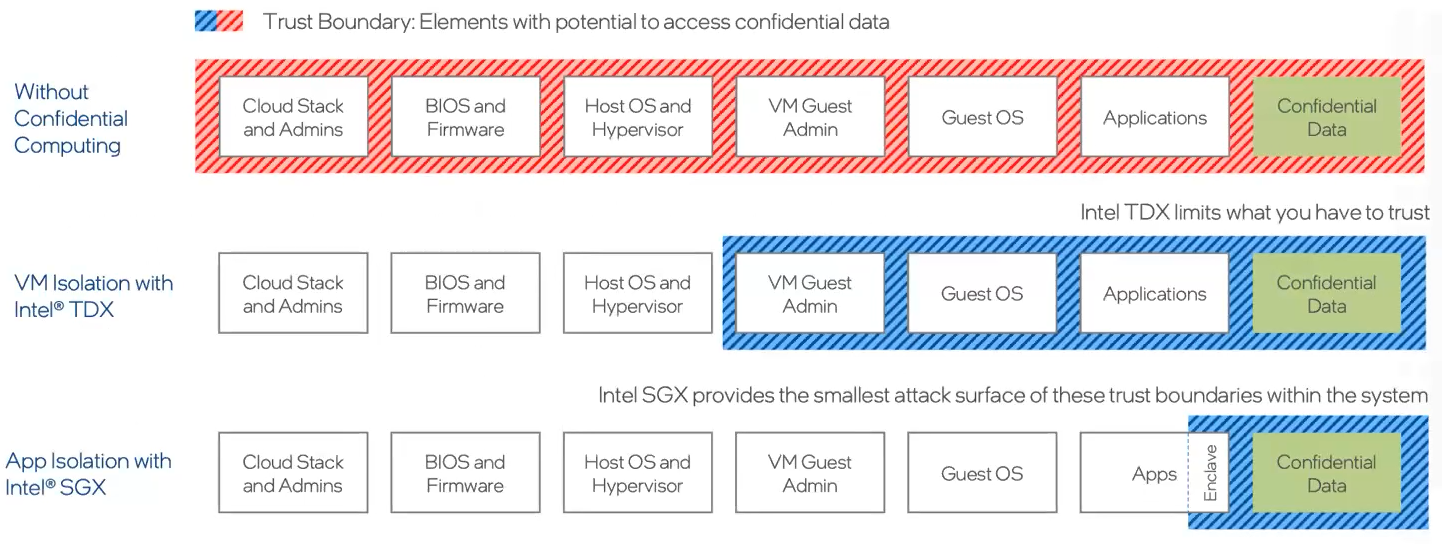
\includegraphics[width=0.4\textwidth]{img/tdx-boundaries.png}
    \caption{Intel TDX Boundaries}
    \label{fig:tdx boundaries}
\end{figure}

In the image we can see 3 level of boundaries:
\begin{itemize}
    \item \textbf{No protection} at all, all the elements can potential access confidential data.
    \item VM protection with \textbf{TDX} provide protection and isolation for all the part related to the virtualized environment.
    \item VM protection with \textbf{SGX}, that provide security principally to the confidential data (the memory storage and just a part of the execution environment with the enclave)
\end{itemize}

\section{Secure Arbitration Mode (SEAM)}

To help enforce the security policies for Trusted Domains, and for support Intel TDX module, a new CPU mode called Secure Arbitration Mode (SEAM) has been introduced.\\ SEAM hosts an Intel-provided, digitally-signed but not encrypted, security service module. \bigskip

The Intel-TDX module, when activated, is hosted in a reserved memory space identified by the SEAM-range register (SEAMRR). \\ The CPU allows access to the SEAM memory range exclusively to software executing inside the SEAM range itself, while excluding all other software and Direct Memory Access (DMA). \bigskip

SEAM is also designed to avoid any memory access privileges to other protected memory regions in the platform. Furthermore, all CPUs capable of SEAM mode are compatible with Intel TDX.

\section{Intel TDX Architecture}

\begin{figure}[H]
    \centering
    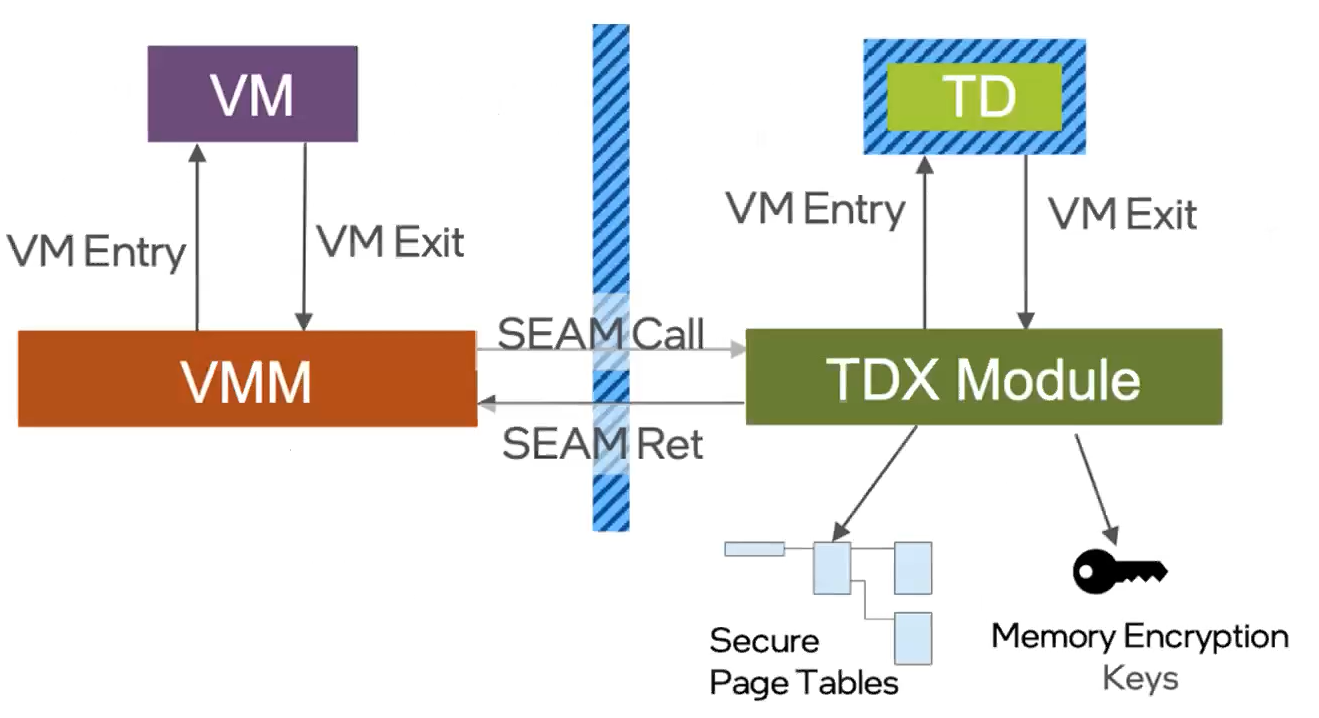
\includegraphics[width=0.4\textwidth]{img/intel tdx arch.png}
    \caption{Intel TDX Architecture}
    \label{fig:tdx arch}
\end{figure}

In the image \ref{fig:tdx arch} the isolation between the normal mode (at the left) and the TDX mode (at the right) which is in charge of deploying as a secure interface for the VMM, the various secure virtual machines called \textbf{TD}. \\
This is done through the help with the help of secure page tables, and memory encryption keys.

\section{Intel TDX Module Tasks \& Instructions}

The \textbf{SEAMCALL} instruction places the CPU in \textit{SEAM-VMX-root} operation and invokes the installation of the TDX module, which provides a secure interface to the Virtual Machine Manager (VMM) for managing TDs.
Acting as a trusted intermediary, the Intel TDX module helps enforce security policies, perform actions, and apply necessary mitigations for TDs, more practically:
\begin{itemize}
    \item It prevents VMM and hypervisor or untrusted entities from accessing registers, performance counters, etc.
    \item It saves and scrubs register states during TD exits to prevent data leakage (state preservation and memory sanitification).
    \item Allows VMM to restrict features for each TD.
\end{itemize}

For remote attestation, the \textbf{SEAMREPORT} instruction is employed to create cryptographic reports. \\ The \textbf{SEAMRET} instruction in introduced to securely returns control to the VMM.


\section{TDX capabilities}
\begin{itemize}
    \item Memory Confidentiality and Integrity
    \item Address-Translation Integrity
    \item CPU-State Confidentiality and Integrity
    \item Remote Attestation
    \item VM preserving updates
\end{itemize}

\subsection{Memory Confidentiality and Integrity}
TDX adopt \textbf{MKTME} (Multi Key Total Memory Encryption) for provide memory confidentiality protection with AES-128-XTS- (or 256). \\
It can operate in 2 modes:
\begin{itemize}
    \item \textbf{cryptographic-integrity scheme:} It's the more secure one, that use a SHA-3-256 hash (\textit{truncated to 28bit !}) for each cache line (64KB) in addition to the encryption. 
            It also have a 1-bit TD ownership tag for each cache line that indicates when a cache line is associated with a memory page assigned to a TD.
    \item \textbf{Logical-integrity mode:} Used for cache line that no need cryptographic integrity protection, it only use the TD ownership tag.
\end{itemize}

\subsubsection{Key Managment}
There are 3 main keys used by TDX:
\begin{itemize}
    \item \textbf{Memory Encryption Key}: As alredy seen, is an AES-128-XTS-Ephemeral (or 256) key used to encrypt the memory of each TD. 
            It is identified by a unique \textbf{KeyID} (HKID) specific for each TD, and can be used only by TDX module and CPU. KeyID can refer also to public keys used in shared memory portions external to TDs.
    \item \textbf{MAC key}: It used only by the CPU to provide integrity protection to the TD measurements report with HMAC-SHA-384.
    \item\textbf{ Attestation key}: (ECDSA 384) Used to sign the attestation report, it's generated and managed by the SGX TD-quoting enclave that is the only one who has access to it.
\end{itemize}

\subsection{Address-Translation Integrity}
Each TD have access to 2 class of memory, a private one that holds the confidential data fo the TD, and a shared one used to communicate with untrusted entities. \\
Both the type of memory have the MSB of the gust-physical address designed as a "Shared" bit, to indicates if the memory is shared (0) or private (1). \\
Moreover, the VMM helps allocate and map memory used by the TDs into the guest physical address to translate them in the host physical addresses of the platform using extended page tables (EPT). 
There are 2 types of EPT, a secure one that is in charge of providing the translation for the private part of the memory for each TD and a shared one related to the public part of the memory (See image \ref{fig:addrs transalation integrity}).

\begin{figure}[H]
    \centering
    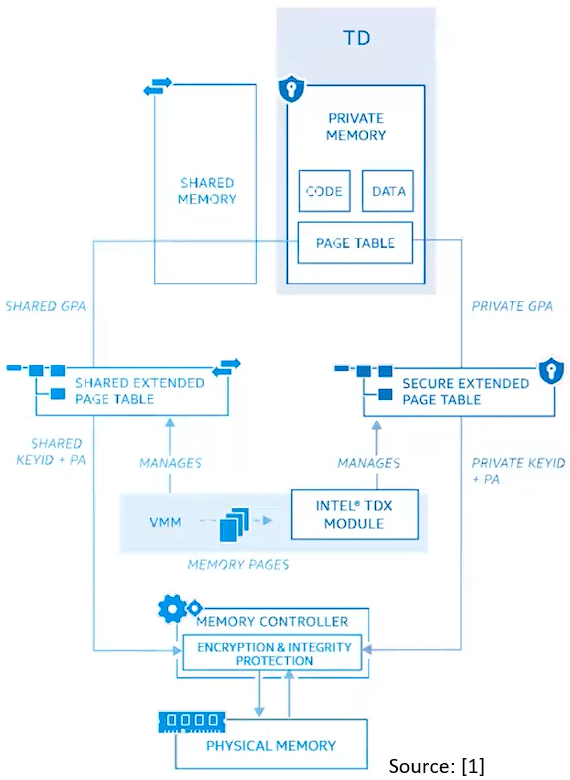
\includegraphics[width=0.4\textwidth]{img/addrs transalation integrity.png}
    \label{fig:addrs transalation integrity}
\end{figure}

The CPU prevents a TD from locating page table structure and executable confidential code in the shared memory by causing page faults in case of errors. \\
Intel TDX has also a tracking system for the extended page tables that is the physical address metadata table and it helps secure page table of a TD to not be allocated in another secure extended page table of another TD.


\subsection{CPU-State Confidentiality and Integrity}
When a TD is created, the module for Intel TDX would require the VMM to provide a set of memory pages to be used to host the virtual-machine-control-structures (VMCS). \\
The goal of the module is to use its page-allocation trackers to enforce that these pages have not been simultaneously assigned to other TDs by the VMM. \\
The Intel-TDX module would then initialize and configure these structures using the TD-assigned, private key to help provide cryptographic confidentiality and integrity protection to the TD-CPU state.


\subsection{Remote Attestation}
Remote attestation is the process that helps a relying party be sure that a software is running on a TD, on a genuine system at a given level of security. TD has two types of measurement register:
\begin{itemize}
    \item \textbf{MRTD}: (measurement register for TD) Provide static measurements for the TD during the build process and contains also the configuration of it.
    \item \textbf{MTMR}: (runtime measurement register) Is an array of four general purpose register used for measurements made at runtime.
\end{itemize}
The method used to take the measurements is the same as for TCB-PCRs, a cumulative SHA-384 hash. \\
The process start from inside the TD (with a specific intruction) that ask to the TDX module to create a specific report structure in which we have the measurements, configuration and measurements of the TD, and also configuration of the TCB, so the intel TDX module. Note that report data value is designed to contain the nonce for the remote attestation process to maintain its freshness. \\
The report generated with this initial part of the remote attestation is marked with the HMAC SHA-384 key

\begin{figure}[H]
    \centering
    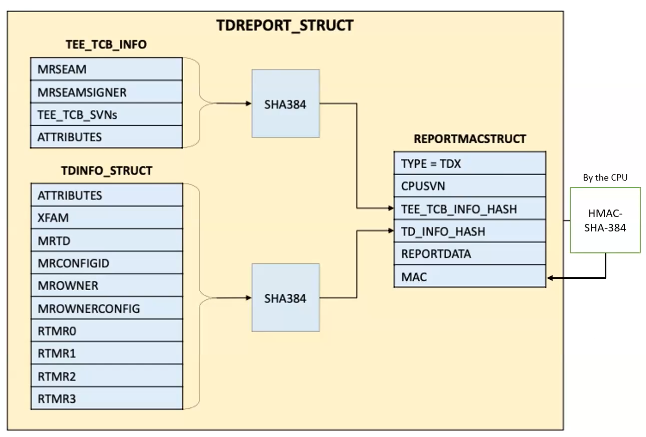
\includegraphics[width=0.4\textwidth]{img/report struct.png}
    \caption{Report Structure}
    \label{fig:report struct}
\end{figure}

The second part of the Remote Attestation is the generation of the quote, that is generated by a specific Intel-SGX enclave called TD-quoting enclave (TDQE) (is in charge of signing the report data, the report for the TD with its own attestation key).
After the report is created, the report is passed to the TD Quoting Enclave through the VMM, that with the inscruction \textbf{EVEIFYREPORT} in able to chec kthe integrity of the report by asking directly to the CPU to make it for him.  If the integrity check is successful, the report is signed with an elliptic curve DSA-384 attestation key. NOTE: The public key certificate related to the TD Quoting Enclave attestation key is issued and signed by Intel itself. \bigskip

The quote verification phase can be done by any party: a relying party or a service inside the cloud service provider. And it can be done: in a secure way inside the Intel SGX Enclave or in an unprotected manner. 
(the verifier is in charge of verifying the measurements and the quote and accept or not the quote).


\begin{figure}[H]
    \centering
    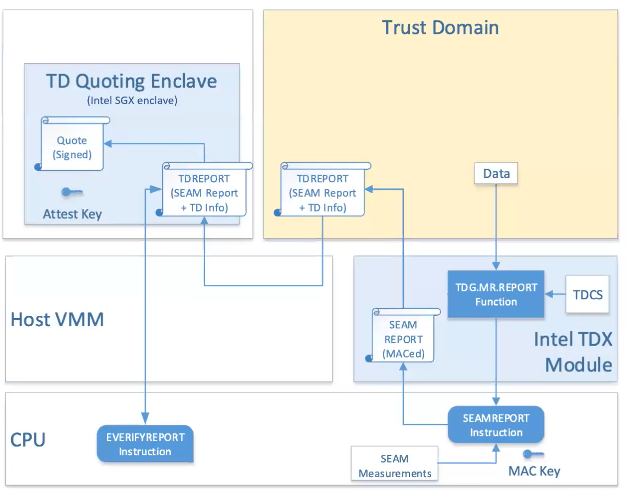
\includegraphics[width=0.4\textwidth]{img/schema tdx attestation.png}
    \caption{scheme representing the internal flow inside the Intel TDX module for attestation}
    \label{fig:schema tdx attestation}
\end{figure}

\subsection{VM preserving updates}
Another feature is the capability of Intel TDX module, to provide update at runtime while persisting TD state and with a minimum TD interruption. (particulary useful for cloud environment). \\
When the TCB linked to each TD will be restored, and a new TCB, associated with the updated TDX Module, will be utilized during the launch of the new TD(s), followed by the subsequent attestation. \\
Existing TDs and their relevant metadata state will be securely saved in encrypted memory owned by the authenticated code module thus protecting the secure surface. \\
TD Preserving Update Flows furnishes updates in orders of milliseconds, this making the 99.999\% Cloud availability goal of CSPs attainable. \\


\section{Threat Model Overview}
There are 2 main adveraries:
\begin{itemize}
    \item \textbf{System software adversary:}  can be insiders of the platform. So developers, but also VMM BIOS, trying to execute malicious software to steal confidential data.
    \item \textbf{Physical adversary:} Someone that access directly access to the platform. That trying to perform hardware attack.
\end{itemize}

\begin{figure}[H]
    \centering
    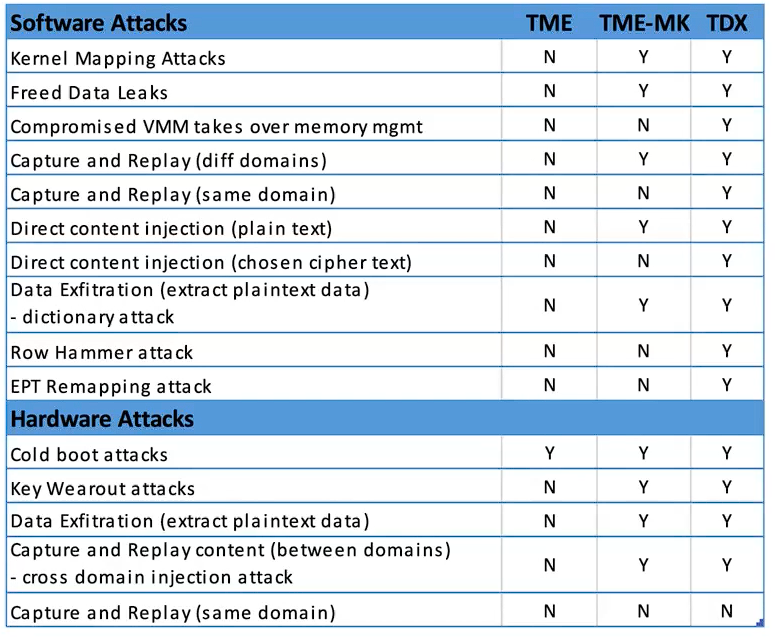
\includegraphics[width=0.4\textwidth]{img/tdx attacks table.png}
    \caption{Table of attacks that TDX can mitigate}
    \label{fig:tdx attacks table}
\end{figure}